\begin{jointwork}
	This thesis builds upon the bachelors project "Online Marketplace Simulation: A Testbed for Self-Learning Agents"
	of the Enterprise Platform and Integration Concepts research group at the Hasso-Plattner-Institute. Therefore, the project will
	be referenced and all examples and experiments will have been conducted using its framework.
\end{jointwork}

\section{Objective of the Thesis}

This thesis introduces ways to monitor the \emph{Reliability} and \emph{Robustness} of different agents (rule-based as well as trained using
various Reinforcement-Learning (RL) approaches) tasked with dynamically pricing products in a Circular Economy marketplace. Since the terms \emph{Reliability}
and \emph{Robustness} can be interpreted differently depending on context and personal experience, we will define our usage in the
\nameref{subsection:ReliabilityAndRobustness} section.
Following the term definitions, we will give a short introduction ans explanation of what a Circular Economy market is (\nameref{subsection:CircularEconomy}) as well as
what Reinforcement Learning is and how we employ the technique in our framework (\nameref{subsection:ReinforcementLearningIntroduction}).

\subsection{Reliability and Robustness}\label{subsection:ReliabilityAndRobustness}

\begin{enumerate}
	\item \emph{Reliability}: With \emph{Reliability}, we describe the ability of an agent to be able to transfer knowledge of a certain type of marketplace and/or
	      against a certain opponent over to a different scenario. If Agent A performs well against Agent B on marketplace M, does it perform the same against Agent C on
	      marketplace M, or against Agent B on marketplace N?

	\item \emph{Robustness}: \emph{Robustness} is the property that describes how well an agent performs over a longer period of time. In a real-world marketplace,
	      consistency is key to success, so finding profitability outliers and their causes are a central part of evaluating an agent's Robustness.
\end{enumerate}

\section{Introduction to the Recommerce platform}

\subsection{The Circular Economy model}\label{subsection:CircularEconomy}
The main goal of the aforementioned bachelors project was to develop a realistic online marketplace that simulates
a Circular Economy. A market is most commonly referred to as being a "Circular Economy" if it includes the three
activities of reduce, reuse and recycle \cite{circularEconomyDefinition}. This means that while in a classical
Linear Economy market each product is being sold once at its \emph{new price} and after use being thrown away,
in a Circular Economy, recycling and thereby waste reduction is a major focus. In our project, we modelled this by
adding two additional price channels, \emph{re-buy price} and \emph{used price}, to the pre-existing \emph{new price} of a product.

The \emph{re-buy price} is defined as the price a vendor is willing to pay a customer to buy back a used product, while the
\emph{used price} is defined as the price the vendor sets for products they previously bought back and now want to sell alongside new products
(whose price is defined by the \emph{new price}).

From now on, we will refer to the Circular Economy market simply as \emph{the market}.

\subsection{Using the simulated marketplace to train agents}\label{subsection:ReinforcementLearningIntroduction}

After the initial market was modelled the goal was to train agents using different reinforcement-learning algorithms
to dynamically set prices on this marketplace, both in monopolistic scenarios as well as in competition with rule-based vendors
which set prices following a strict set of pre-defined rules. \todo{Is the following sentence a footnote?}These rules can range from simply undercutting the
lowest competitor's price to more advanced techniques such as price-fixing and -gouging.\todo{find out if we have such competitors}

% hbt! tells Latex to not put the figure at the top/bottom/newpage but exactly where defined
\begin{figure}[hbt!]
	\centering
	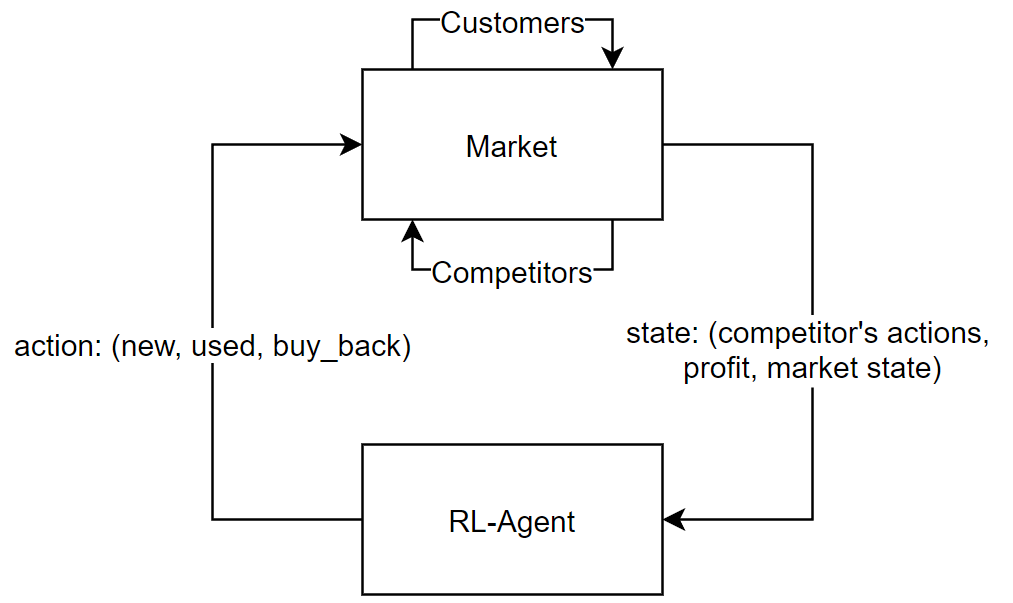
\includegraphics[height = 7 cm]{images/RL-Overview.png}\\[1 ex]
	\caption{The standard reinforcement-learning model in the context of our market.}
	\label{fig:IntroRLDiagram}
\end{figure}

Reinforcement-learning agents are trained through a process of trial-and-error. They interact with the market through an observable state
and an action which influences the following state. \Cref{fig:IntroRLDiagram} illustrates the RL-model in the context of our
market.\todo{Create a \emph{nicer} diagram with the three prices} The goal of the agent is to maximize the so-called reinforcement signal,
which in our case is the profit the agent made during the last cycle, since we want to train agents to maximize profits on real markets.
By observing which prices lead to which reinforcement signal, the agents get more profitable over the course of training.
